\subsection{Model with truncated gaussian kernel}

In this section is now presented the choice of the model made to study the possible influence of a determinist point process $e_p$ on a temporal point process $z_k$, where $e_p$ and $z_k$ correspond to specific data in the context of electrophysiology, as mentioned above.
Several choices and assumptions are made in order to obtain the model presented below, those are detailed and explained later in Section~\ref{hypotheses}, in particular concerning the choice of the kernel shape.

When driven by $e_p$, the dynamic of $z_k$'s counting process $N_t^{(k)} \coloneqq \sum_{t_k \in \mathcal{A}_k} \1[t_k \leq t]$ can be describe by its intensity: $\forall t\in\intervalleFF{0}{T}$,
\begin{equation}\label{eq:intensity_definition}
    \lambda_{k,p}(t) \equiv \lambda_{k}\pars{t \middle| \mathscr{F}_t^{(p)}} \coloneqq \lim_{\dint t \xrightarrow{} 0 }\frac{\proba{N_{t+\dint t}^{(k)} - N_t^{(k)} = 1}[\mathscr{F}_t^{(p)}]}{\dint t}
\end{equation}
where $\mathscr{F}_t^{(p)} = \enstq{t_i \in t^{(p)}}{t_i < t}$ is the information available on $e_p$ up to, but not including, $t$.

\paragraph{Our model} As previously mentioned, the shape of the intensity is derived from the Hawkes process model, with a baseline intensity and a kernel function.
Note that here again, we consider the link function to be the identity function.
Namely,

\begin{equation}\label{eq:model_intensity}
    \lambda_{k,p}(t)  = \mu_k + \alpha_{k,p}\kappa_{k,p}(t - t_*^{(p)}(t))\1[t \geq t_1^{(p)}]
\end{equation}
where $t_*^{(p)}(t) \coloneqq \max\enstq{t'}{t' \in t^{(p)}, t' \leq t}$ denotes the timestamp of the last task of type $p$ occurred before ($\leq$) time $t$, $\alpha_{k,p}\in\R$ is a coefficient determining the relative importance of the stimulus $p$ in the activation of the atom $k$, and where $\kappa_{k,p}$ is the probability density function of a truncated gaussian distribution of mean $m_{k,p}\in\R$ and standard deviation $\sigma_{k,p}>0$, with truncation values $\intervalleFF{a}{b}\in\R$, noted $\Norm[\bracks{a,b}]{m_{k,p}}{\sigma_{k,p}^2}$, namely,
\begin{equation}\label{eq:kernel_trunc_norm}
    \kappa_{k,p}(x) \equiv \kappa(x ; m_{k,p}, \sigma_{k,p}, a, b)=\frac{1}{\sigma_{k,p}} \frac{\phi\left(\frac{x-m_{k,p}}{\sigma_{k,p}}\right)}{\Phi\left(\frac{b-m_{k,p}}{\sigma_{k,p}}\right)-\Phi\left(\frac{a-m_{k,p}}{\sigma_{k,p}}\right)} \1[a\leq x\leq b]
\end{equation}
where
$$
\phi(x) = \frac{1}{\sqrt{2\pi}}\exp\left(-\frac{1}{2}x^2\right)
$$ 
is the probability density function of the standard normal distribution, and
$$
\Phi(x) = \frac{1}{\sqrt{2\pi}} \int_{-\infty}^x \exp\left(-\frac{1}{2}t^2\right) \mathrm{d}t
$$
is its cumulative distribution function.

Note that by definition, if $b=\infty$, then $\Phi\left(\frac{b-m_{k,p}}{\sigma_{k,p}}\right) = 1$, and similarly, if $a=-\infty$, then $\Phi\left(\frac{a-m_{k,p}}{\sigma_{k,p}}\right) = 0$.
An example of a truncated normal distribution is presented in Fig.~\ref{fig:trunc_norm_distribution}.

\begin{figure}[h!]
    \centering
    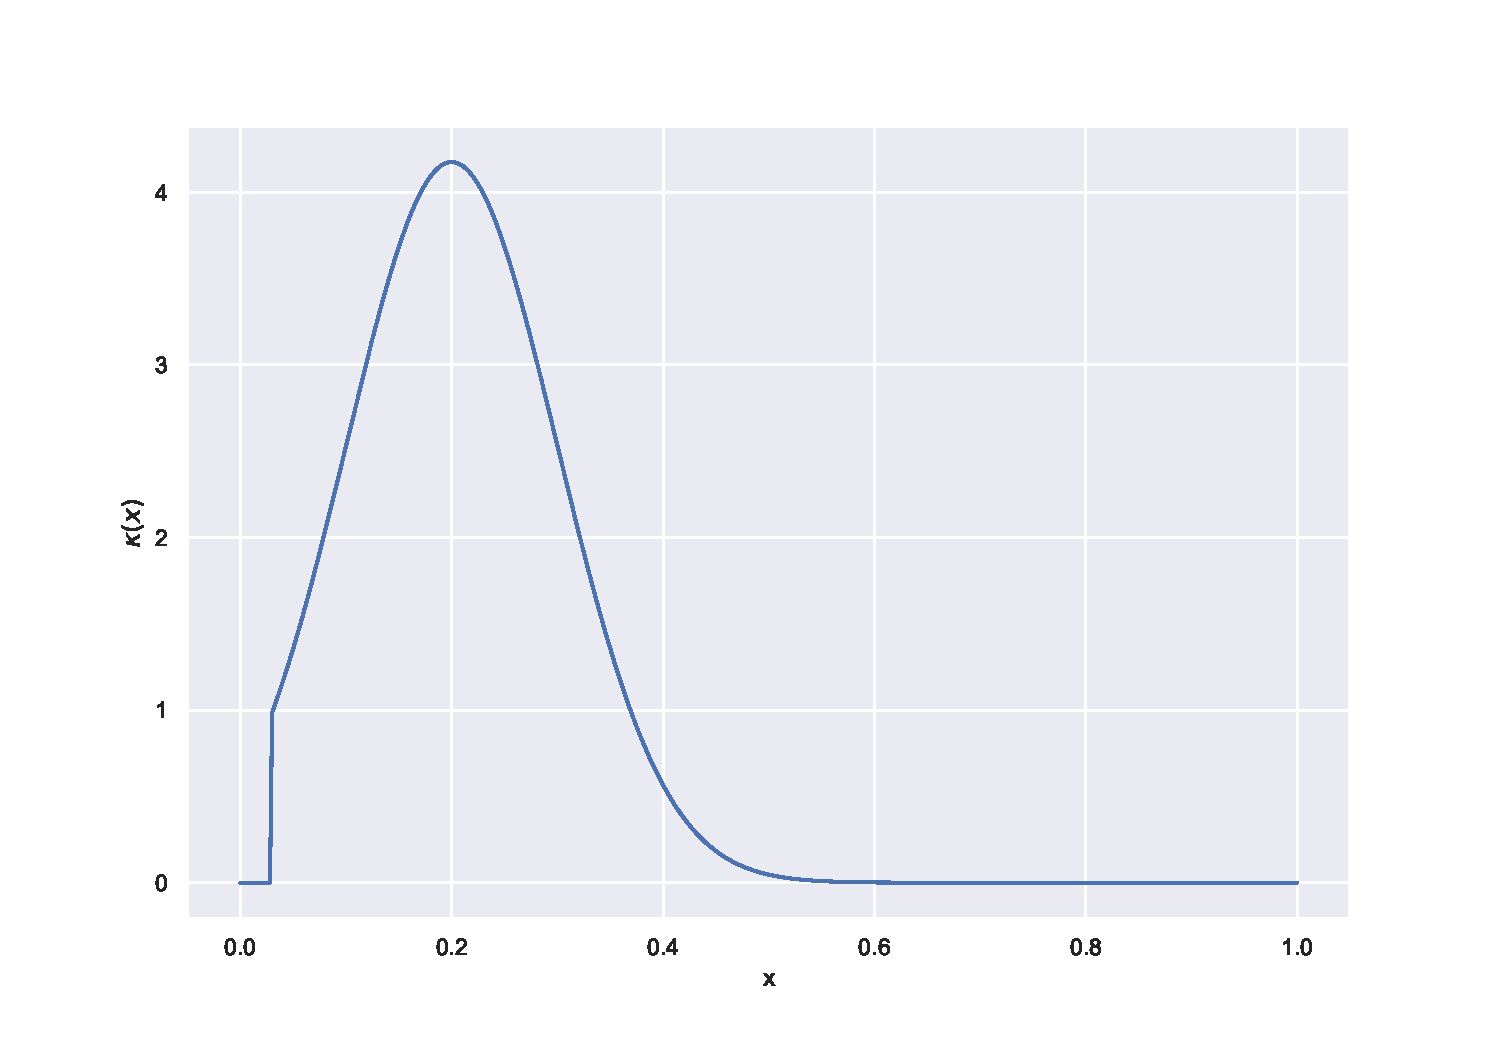
\includegraphics[width=0.9\textwidth]{pics/trunc_norm_distribution.pdf}
    \caption{Truncated Normal distribution with $m=\num{0.2}$, $\sigma=0.1$, $a=0.03$ and $b=0.8$.}
    \label{fig:trunc_norm_distribution}
\end{figure}